%f%%%%%%%%%%%%%%%%%%%%%%% file template.tex %%%%%%%%%%%%%%%%%%%%%%%%%
%
% This is a general template file for the LaTeX package SVJour3
% for Springer journals.          Springer Heidelberg 2010/09/16
%
% Copy it to a new file with a new name and use it as the basis
% for your article. Delete % signs as needed.
%
% This template includes a few options for different layouts and
% content for various journals. Please consult a previous issue of
% your journal as needed.
%
%%%%%%%%%%%%%%%%%%%%%%%%%%%%%%%%%%%%%%%%%%%%%%%%%%%%%%%%%%%%%%%%%%%
%
% First comes an example EPS file -- just ignore it and
% proceed on the \documentclass line
% your LaTeX will extract the file if required
\begin{filecontents*}{example.eps}
%!PS-Adobe-3.0 EPSF-3.0
%%BoundingBox: 19 19 221 221
%%CreationDate: Mon Sep 29 1997
%%Creator: programmed by hand (JK)
%%EndComments
gsave
newpath
  20 20 moveto
  20 220 lineto
  220 220 lineto
  220 20 lineto
closepath
2 setlinewidth
gsave
  .4 setgray fill
grestore
stroke
grestore
\end{filecontents*}
%
\RequirePackage{fix-cm}
%
%\documentclass{svjour3}                     % onecolumn (standard format)
%\documentclass[smallcondensed]{svjour3}     % onecolumn (ditto)
%\documentclass[smallextended,final]{svjour3}       % onecolumn (second format)
\documentclass[twocolumn]{svjour3}          % twocolumn
\usepackage[toc,page]{appendix}
%
\smartqed  % flush right qed marks, e.g. at end of proof
%
\let\proof\relax 
\let\endproof\relax
\usepackage{times}
%\usepackage{natbib}
\usepackage{helvet}
\usepackage{courier}
\usepackage{comment}
\usepackage{subcaption}
\captionsetup{compatibility=false}
\usepackage{wrapfig}
\usepackage{float}
%\usepackage{subcaption}
\usepackage{times}

\usepackage{epsfig}
\usepackage{graphicx}
\usepackage{amsmath}
\usepackage{wrapfig}
\usepackage{amssymb}
\usepackage{comment}
%\usepackage{caption}
\usepackage[font=small,labelfont=bf]{caption}
\usepackage{enumi tem}
\newcommand{\ignore}[1]{}
\usepackage[noend]{algorithm2e}
\usepackage{algorithmicx,algpseudocode}
\usepackage{booktabs,tabularx}%
\usepackage{multirow} 
\usepackage{amsthm}
\theoremstyle{plain}
\linespread{1.0}
\theoremstyle{definition}
\newtheorem{thm}{Theorem}[section]
\newtheorem{lem}[thm]{Lemma}
\newtheorem{prop}[thm]{Proposition}
\newtheorem*{cor}{Corollary}
\theoremstyle{definition}
\newtheorem{defn}{Definition}[section]
\newtheorem{conj}{Conjecture}[section]
\newtheorem{exmp}{Example}[section]
\theoremstyle{remark}
\newtheorem*{rem}{Remark}
%\graphicspath{{../BMVC15_camera_ready/}{../BMVC15_camera_ready/images/}{../BMVC15_camera_ready/supp2015_camera_ready/}}
%\usepackage{graphicx}
%\usepackage{amsmath,amssymb} % define this before the line numbering.
%\usepackage{ruler}
%\usepackage{color}
%\usepackage{expl3}
%\renewcommand\baselinestretch{0.98}
%\usepackage[width=122mm,left=12mm,paperwidth=146mm,height=193mm,top=12mm,paperheight=217mm]{geometry}

\def\ignore#1{}

%\ExplSyntaxOn
%\newcommand\latinabbrev[1]{
%  \peek_meaning:NTF . {% Same as \@ifnextchar
%    #1\@}%
%  { \peek_catcode:NTF a {% Check whether next char has same catcode as \'a, i.e., is a letter
 %     #1.\@ }%
%    {#1.\@}}}
%\ExplSyntaxOff

\def\onedot{.}
\def\eg{\emph{e.g}\onedot~} \def\Eg{\emph{E.g}\onedot}
\def\ie{\emph{i.e}\onedot~} \def\Ie{\emph{I.e}\onedot}
\def\cf{\emph{c.f}\onedot} \def\Cf{\emph{C.f}\onedot}
\def\etc{\emph{etc}\onedot} \def\vs{\emph{vs}\onedot}
\def\wrt{w.r.t\onedot} \def\dof{d.o.f\onedot}
\def\etal{\emph{et al}~}

\let\oldemptyset\emptyset
\let\emptyset\varnothing

%\AtBeginDocument{%
%  \setlength{\oddsidemargin}{\dimexpr(\paperwidth-\textwidth)/2-1in}%
%  \setlength{\evensidemargin}{\oddsidemargin}%
%  \setlength{\topmargin}{%
%    \dimexpr(\paperheight-\textheight)/2-\headheight-\headsep-1in}%
%}
%
% \usepackage{mathptmx}      % use Times fonts if available on your TeX system
%
% insert here the call for the packages your document requires
%\usepackage{latexsym}
% etc.
%
% please place your own definitions here and don't use \def but
% \newcommand{}{}
%
% Insert the name of "your journal" with
% \journalname{myjournal}
%

\begin{document}

%\title{Overlapping Domain Cover for  Scalable  and Accurate Regression Kernel Machines }


\title{Overlapping Cover Local Regression Machines }

%\thanks{Grants or other notes
%about the article that should go on the front page should be
%placed here. General acknowledgments should be placed at the end of the article.}

%\subtitle{from Pure Text or weak Attributes}

\author{Mohamed Elhoseiny    \and
        Ahmed Elgammal     %etc.
}

\authorrunning{M Elhoseiny et al.}
%\authorrunning{Short form of author list} % if too long for running head

\institute{Mohamed Elhoseiny$^{1}$ and Ahmed Elgammal$^{2}$ \at
	       $^{1}$Facebook AI Research\\
	       $^{2}$Department of Computer Science, Rutgers University\\
             % 110 Frelinghuysen Road, Piscataway, NJ 08854-8019, USA \\
              %USA\\
              %Tel.: +1-732-208-9712\\	
              \email{elhoseiny@fb.com, elgammal@cs.rutgers.edu}           %  \\
%             \emph{Present address:} of F. Author  %  if needed
       %    \and
        %   Ahmed Elgammal \at
         %  110 Frelinghuysen Road, \\ 
         %  Piscataway, NJ 08854-8019 \\
         %  USA\\
         %  \email{elgammal@cs.rutgers.edu}          
}


\date{Received: date / Accepted: date}
% The correct dates will be entered by the editor


\maketitle


\begin{abstract}


%\ignore{Based on this notion, we propose an ODC framework that could be applied to various kernel machines, \eg Gaussian Process Regression(GPR)  and Twin Gaussian Processes (TGP). The framework was evaluated on POSER, Human Eva and Human3.6M datasets. The results indicate accurate and fast prediction are  achieved by the proposed framework on both GPR and TGP. We also achieved quadratic prediction complexity for TGP instead of cubic complexity in prior work. }
%\ignore{Regression in large scale systems has been a very challenging task with many applications in pattern recognition and computer vision.} In this paper, we present the Overlapping Domain Cover (ODC) notion for kernel machines, as a set of overlapping subsets of the data that covers the entire training set and optimized to be spatially cohesive as possible. We showed the value of this notion for overlapping local kernel machines for regression in terms of speed and accuracy. \ignore{Adopting this notion,} We propose an ODC framework that reduces the computational complexity of \ignore{the local scheme in} Twin Gaussian Processes (TGP) regression from cubic to quadratic in the number of points in the local kernel machine. Our ODC framework also is scalable in the number of dimensions of the input domain which is a limitation is some method in the literature. It is also applicable to other  regression methods (\eg   Gaussian Process Regression(GPR) and IWTGP regression), as shown in our experiments. We validated and analyzed the parameters of our framework on three Human 3D pose estimation datasets and interesting findings are been discussed.

%\ignore{
%In this paper, we present the Overlapping Domain Cover (ODC) notion for kernel machines, as a set of overlapping subsets of the data that covers the entire training set and optimized to be spatially cohesive as possible. We showed the value of this notion in local kernel machines for regression in terms of speed and accuracy. We propose an ODC framework that reduces the computational complexity of Twin Gaussian Processes (TGP) regression from cubic to quadratic in the number of points in the local kernel machine. Our ODC framework also is scalable in the number of dimensions of the input domain which is a limitation is some method in the literature. It is also applicable to other  regression methods (\eg   Gaussian Process Regression(GPR) and IWTGP regression), as shown in our experiments. We validated and analyzed the parameters of our framework on three Human 3D pose estimation datasets and interesting findings are  discussed.}

We present the Overlapping Domain Cover (ODC) notion for kernel machines, as a set of overlapping subsets of the data that covers the entire training set and optimized to be spatially cohesive as possible. We show how this notion benefit the speed of local kernel machines for regression in terms of both speed while achieving while minimizing the prediction error. We propose an efficient ODC framework, which is applicable to various regression models and in particular reduces the complexity of Twin Gaussian Processes (TGP) regression from cubic to quadratic. Our notion is also applicable to several kernel methods (\eg   Gaussian Process Regression(GPR) and IWTGP regression, as shown in our experiments). We also theoretically justified the idea behind our method to improve local prediction by the overlapping cover. We validated and analyzed our method on three benchmark human pose estimation datasets and interesting findings are discussed.  

%Section 4, presents an idea of how to build a domain decomposition TGP 

\end{abstract}
\section{Introduction}
\label{sec:1}

\ignore{One of the main problems, in many computer vision application, is to estimate a continuous real-valued function or a structured-output function from input features.} Estimation of a continuous real-valued or a structured-output function from input features is one of the critical problems that appears  in many machine learning  applications. Examples include predicting the joint angles of the human body from images, head pose, object viewpoint, illumination direction, and a person's age and gender. Typically, these problems are formulated by a regression model.  Recent advances in structure regression encouraged researchers to adopt it for formulating various problems with high-dimensional output spaces, such as segmentation, detection, and image reconstruction, as regression problems. However, \ignore{they are constrained by }the computational complexity of the state-of-the-art regression algorithms limits their applicability for big data\ignore{ that are used to compute the predictions}. In particular,  kernel-based regression algorithms such as Ridge Regression~\cite{ridgeReg70}, Gaussian Process Regression (GPR)~\cite{Rasmussen:2005}, and the Twin Gaussian Processes (TGP)~\cite{Bo:2010} require inversion of kernel matrices ($O(N^3)$, where $N$ is the number of the training points), which limits their applicability for big data. We refer to these non-scalable versions of GPR and TGP as full-GPR and full-TGP, respectively.
 
 %this should move elsewhere.
 %From data bias perspective, Yamada et al \cite{Yamada:2012}, proposed a co-variance shift adaptation algorithm and applied on Kernel regression (KR)~\cite{kernelReg03} and TGP, by incorporating importance weighting to the training points based on the training and test distributions. However, their approach gives the best prediction on TGP, which requires matrix inversion in both its weight and unweighted versions. .   



%Many machine learning tasks are constrained by computational time of the state-of-the-art algorithms, required to compute the prediction. For instance,  Gaussian Process Regression (GPR)~\cite{Rasmussen:2005}, Ridge Regression \cite{ridgeReg70}, Twin Gaussian Processes (TGP)~\cite{Bo:2010} which require inversion of Kernel matrices ($O(N^3)$, $N$ is the number of the training points ), which limits its applicability for large scale data. From data bias perspective, Yamada et al \cite{Yamada:2012}, proposed a co-variance shift adaptation algorithm and applied on Kernel regression (KR)~\cite{kernelReg03} and TGP, by incorporating importance weighting to the training points based on the training and test distributions. However, their approach gives the best prediction on TGP, which requires matrix inversion in both its weight and unweighted versions.

%\begin{figure}{r}{0.43\textwidth}
\begin{comment}
\begin{figure}
%\centering
%\begin{tabular}{cc}
%\bmvaHangBox{\fbox{
\includegraphics[width=0.21\textwidth]{nonOverlappingFig.png}
%\bmvaHangBox{\fbox{
\includegraphics[width=0.21\textwidth]{OverlappingFig.png}%\\
%(a)&(b)s
%\end{tabular}
\caption{24 points, Left: 3 disjoint kernel machines of 8  points,  Right: 5 Overlapping kernel machines of 8 points. $f_i(\mathbf{x}^*)$ is the $i^{th}$ kernel machine prediction for $\mathbf{x}^*$ test point.}
\label{fig:overlapandnonoverlap}
\end{figure}
\end{comment}




Khandekar et. al. \cite{khandekar2014advantage} discussed properties and  benefits of overlapping clusters for minimizing the conductance from spectral perspective. These properties of overlapping clusters also motivate studying scalable local prediction based on overlapping kernel machines.  Figure~\ref{fig:overlapandnonoverlap_ex} illustrates the notion by starting from a set of points, diving them into either disjoint and overlapping subsets, and finally learning a kernel prediction function on each (i.e., $f_i(x^*)$ for subset $i$, $x^*$ is testing point). \ignore{Our method is accurate and scalable as demonstrated in the experiments on 3-datasets (including Human3.6M, the largest human-3D-pose dataset).}
\textit{In summary, the main question, we  address in this paper, is how local kernel machines with overlapping training data could help speedup the computations and gain accurate predictions. We achieved considerable speedup and good performance on GPR, TGP, and IWTGP (Importance Weighted TGP) applied to 3D pose estimation datasets\ignore{; our framework firstly achieves quadratic prediction complexity for TGPs}. To the best of our knowledge, our framework is the first to achieve quadratic prediction complexity for TGP. The ODC concept is also novel in the context of kernel machines and is shown here to be successfully applicable to multiple kernel-machines\ignore{, resulting in a considerable speedup and an accurate prediction}}. We studies in this work GPR and TGP and IWTGP  (a third model) kernel machines\ignore{ (denoted by SM in the rest of the paper)}. The remainder of this paper is organized as follows: Section ~\ref{sec:2}  and~\ref{sec:relappmethod} presents some motivating kernel machines and the related work. Section ~\ref{sec:3} presents our approach and a theoretical justification for our ODC concept. Section ~\ref{sec:6} and \ref{sec:7} presents our experimental validation and conclusion.

\begin{comment}
There are five main contributions to this paper:
\begin{enumerate}[noitemsep,topsep=0pt,parsep=0pt,partopsep=0pt,leftmargin=*]
\item{Persistent prediction on boundaries is achieved our domain set cover notion.}
\item{As a first step of the (OD) cover computation, we propose a variant of K means algorithm to use for domain decomposition with equal number of points per cluster.}
\item{Our Overlapping Domain Cover notion is not restricted
to GPR. It is applicable various kernel machines (\eg TGP,
kernel regression).}
\item{$O(N^2)$ complexity is achieved for TGP and IWTGP local prediction under our framework.}
\item{We conducted experiments on three 3D-pose estimation datasets to validate our method.}
\end{enumerate}
\end{comment}
\begin{comment}
Section ~\ref{sec:2} present example kernel machines that benefits from our approach. Section ~\ref{sec:} presents an overview of our domain. Section ~\ref{} presents that training phases which involves  
\end{comment}
\begin{comment}
Performance advantages of our approach are detailed in the experiential results section. The remaining of this paper is organized as follows. Section 2 presents The domain decomposition framework, Section 3 and 4 detail the training and prediction phases. Section 5 presents the IWTGP integration under our framework. Section 6 presents experimental results. Finally, Section 7 presents the conclusion and future work.
\end{comment}
%\begin{figure}[t!]
%\centering
%    \begin{subfigure}[b]{0.19\textwidth}
%    \includegraphics[width=1.0\textwidth,height=0.75\textwidth]{nonOverlappingFig.png}
%    \vspace{-5mm}
%               \caption{$\,\,$}
%                \label{fig:nonoverlapping}
%        \end{subfigure}%
%        \begin{subfigure}[b]{0.19\textwidth}
%   \includegraphics[width=1.0\textwidth,height=0.75\textwidth]{OverlappingFig.png}
%       \vspace{-5mm}
%                \caption{$\,\,$}
%                 \label{fig:overlapping}
%        \end{subfigure}
%        \vspace{-4mm}
%        \caption{24 points (a) 3 disjoint kernel machines of 8  points, (b) 5 Overlapping kernel machines of 8 points. $f_i(\mathbf{x}^*)$ is the $i^{th}$ kernel machine prediction for $\mathbf{x}^*$ test point.}
%        \label{fig:overlapandnonoverlap}
%           \vspace{-6mm}
%\end{figure}


%\begin{figure}
%\centering
%\begin{tabular}{cc}
%\bmvaHangBox{\fbox{
%\includegraphics[width=2.8cm]{nonOverlappingFig.png}}}&
%\bmvaHangBox{\fbox{\includegraphics[width=2.8cm]{OverlappingFig.png}}}\\
%%\bmvaHangBox{\fbox{\includegraphics[width=5.6cm]{OverlappingFig.png}}}\\
%(a)&(b)
%\end{tabular}
%\caption{24 points (a) 3 disjoint kernel machines of 8  points, (b) 5 Overlapping kernel machines of 8 points. $f_i(\mathbf{x}^*)$ is the $i^{th}$ kernel machine prediction for $\mathbf{x}^*$ test point.}
%\label{fig:overlapandnonoverlap}
%\end{figure}

\begin{figure*}[t]
\centering
%\centering
%\begin{tabular}{cc}
%\bmvaHangBox{\fbox{
\includegraphics[width=0.31\textwidth]{ODC_intro_1.png}
%\bmvaHangBox{\fbox{
\includegraphics[width=0.31\textwidth]{ODC_intro_2.png}%\\
\includegraphics[width=0.31\textwidth]{ODC_intro_3.png}
\includegraphics[width=0.62\textwidth]{ODC_intro_4.png}
%(a)&(b)s
%\end{tabular}
\caption{\textbf{Top}: Left:24 points, Middle: Overlapping Cover, Right: disjoint kernel machines of 8  points (evaluating $x^*$ near a middle of a kernel machine).  \textbf{Bottom}: Left: disjoint kernel machine evaluation on boundary),  Right: 6 Overlapping kernel machines of 8 points.  $f_i(\mathbf{x}^*)$ is the $i^{th}$ kernel machine prediction for $\mathbf{x}^*$ test point.}
\label{fig:overlapandnonoverlap_ex}
\vspace{-3mm}
\end{figure*}

\section{Background on Full GPR and TGP Models}
\label{sec:2}
In this section, we show example kernel machines that motivated us to propose the ODC framework to improve their performance and scalability.   Specifically, we review GPR for single output regression, and TGP for structured output regression.\ignore{ Specifically, we review two powerful machines for single output (Gaussian Process Regression(GPR)) and structured output regression (Twin Gaussian Processes(TGP)).Then, we present an importance weighting algorithm to resolve data bias under Twin-Gaussian Processes (IWTGP)} We selected GPR and TGP kernel machines for their increasing interest and impact. However, our framework is not  restricted to them\ignore{ as it depends on the overlapping domain cover notion that could be generally adopted}. \ignore{We conclude this section by showing practical limitation of these machines that inspires our method. }

%\subsection{Gaussian Process Regression (GPR)}
%\label{sec:relgpr}



\textbf{GPR}~\cite{Rasmussen:2005}  assumes a linear model in the kernel space with Gaussian noise in a single-valued output, i.e., $y = f(\textbf{x})  + \mathcal{N} (0, \sigma_{n}^2)$, where $\textbf{x} \in \mathbb{R}^{d_X}$ and ${y} \in \mathbb{R}$. Given a training set $\lbrace \textbf{x}_i, {y}_i , i =1:N \rbrace$, the posterior distribution of $y$ given a test point $\textbf{x}_{*}$ is:   \ignore{dimension $i$ of the classifier to be predicted ($\textbf{y}_* \in R^{d_Y}$)}
\begin{comment}
\begin{equation}
y_i = f_i(t) +e_i ,  \,\,\,\,     e_i ∼ \mathcal{N} (0, \sigma_{ni}^2),        
\end{equation}
\end{comment}
\begin{equation}
\small
\begin{split}
p(y|\textbf{x}_*)=   \mathcal{N} (&\boldsymbol{\mu}_{y} =  \textbf{k}{(\textbf{x}_*)}^\top (\textbf{K} + \sigma^2_{n} \textbf{I})^{-1} \mathbf{f},   \\  &  \sigma_{y}^2 = k({\textbf{x}_*, \textbf{x}_*}) -\textbf{k}{(\textbf{x}_*)}^\top (\textbf{K} + \sigma^2_{n} \textbf{I})^{-1} \textbf{k}{(\textbf{x}_*)})
\end{split}
\label{eq:gprpred}
\end{equation}
where $k(\textbf{x},\textbf{x}')$ is kernel defined in the input space, $\mathbf{K}$ is an $N \times N$ matrix, such that $\mathbf{K} (l,m) = k(\textbf{x}_l, \textbf{x}_m)$, $\textbf{k}{(\textbf{x}_*)}  = [k(\textbf{x}_*,\textbf{x}_1),, ..., {k}(\textbf{x}_*,\textbf{x}_{N})]^\top$, $\textbf{I}$ is an  identity matrix of size $N$, $\sigma_{n}$ is the variance of the measurement noise, $\mathbf{f} = [y_1,\cdots  $ $, y_N]^\top$. GPR could predict structured output $\textbf{y} \in \mathbb{R}^{d_Y}$ by training a GPR  model for each dimension\ignore{ $i = 1 : d_Y$}. However, this indicates that GPR does not capture dependency between output dimensions which limit its performance. 
%\subsection{Twin Gaussian Processes (TGP)}
%\label{sec:reltgp}

\textbf{TGP}~\cite{Bo:2010} encodes the relation between both inputs and outputs using GP priors. This was achieved by minimizing the Kullback-Leibler divergence between the marginal GP of outputs (e.g., poses) and observations (e.g., features)\ignore{; we refer the reader to~\cite{Bo:2010} for derivation}. Hence,  TGP prediction is given by:\ignore{ the estimated pose in TGP is given as the solution of the following optimization problem:}
\begin{equation}
\small
\begin{split}
\hat{\textbf{y}}(\textbf{x}_*) =  &\underset{\textbf{y}}{\operatorname{argmin       }}[  k_Y(\textbf{y},\textbf{y})  -2 \textbf{k}_Y(\textbf{y})^\top (\textbf{K}_X + \lambda_X  \textbf{I})^{-1} \textbf{k}_X(\textbf{x}_*) \\&- \eta  log (k_Y(\textbf{y},\textbf{y})  -\textbf{k}_Y(y)^\top ({\textbf{K}_Y}+ \lambda_Y \textbf{I})^{-1} {\textbf{k}_Y(\textbf{y})} ) ]
\end{split}
\label{eq:tgp}
\vspace{-5mm}
\end{equation}
where $\eta  = k_X(\textbf{x}_*,\textbf{x}_*) -\textbf{k}_X(\textbf{x}_*)^\top  (\textbf{K}_X + \lambda_X  \textbf{I})^{-1} \textbf{k}_X($ $\textbf{x}_*)$, $k_X(\textbf{x},\textbf{x}') = exp(\frac{- \|\textbf{x}-\textbf{x}' \|}{2 \rho_x^2})$ and $k_Y(\textbf{y},\textbf{y}')$ $= exp(\frac{- \|\textbf{y}-\textbf{y}' \|}{2 \rho_y^2})$ are Gaussian kernel functions for input feature $\textbf{x}$ and output vector $\textbf{y}$, $\rho_x$ and $\rho_y$ are the kernel bandwidths for the input and the output  . $\textbf{k}_Y(\textbf{y}) = [k_Y(\textbf{y},\textbf{y}_1), ..., k_Y(\textbf{y},\textbf{y}_{N})]^\top$, where $N$ is the number of the training examples. $\textbf{k}_X(\textbf{x}_*) = [k_X(\textbf{x}_*,\textbf{x}_1), ...,$ ${k}_X(\textbf{x}_*,\textbf{x}_{N})]^\top$, and $\lambda_X$ and $\lambda_Y$ are regularization parameters to avoid overfitting. This optimization problem can be solved using a quasi-Newton optimizer with cubic polynomial line search \ignore{for optimal step size selection}~\cite{Bo:2010}; we denote the number of steps to convergence as $l_2$.




\begin{table*}[t!]
\centering
 %\vspace{-5mm}
\caption{Comparison of computational Complexity of training and testing for each of Full, NN (Nearest Neighbor), FITC, Local-RPC, and our ODC. Training is the time include all computations that does not depend on test data, which includes clustering in some of these methods. Testing includes computations only needed for prediction\ignore{performed at test time, i.e., Mean $\textbf{Y}$ and variance for GPR kernel machine and the prediction $\textbf{Y}$ for TGP kernel machine}}
%\vspace{2mm}
 \label{tab:thcomp}
  \scalebox{0.68}{
    \begin{tabular}{|l|ccc|cc|c|}
    %\toprule
    \hline
          &  \multicolumn{3}{c|}{\textbf{Training for GPR and TGP}}    & \multicolumn{3}{|c|}{\textbf{Testing for each point} }  \\ \hline
    %\midrule
          & \textbf{Ekmeans Clustering} & \textbf{RPC Clustering}   &    \textbf{Model training}   & \textbf{GPR-Y} & \textbf{GPR-Var} & \textbf{TGP-Y} \\ \hline 
    \textbf{Full} & -     & -     & $O(N^3 + N^2 d_X)$    & $O(N \cdot (d_X +d_Y)$ & $O(N^2 \cdot d_Y)$ & $O(l_2 \cdot N^2 \cdot d_Y)$ \\
    \textbf{NN {\cite{Bo:2010}}} & -     & -     & -     & $O(M^3 \cdot d_Y)$ & $O(M^3 \cdot d_Y)$ & $O(M^3 + l_2 \cdot M^2 \cdot d_Y)$ \\
    \textbf{FIC (GPR only, $d_Y=1$ {~\cite{fic06}})} & - & - & $O(M^2 \cdot ( {N} + d_X))$  & $O(M \cdot d_X)$  & $O(M^2)$ & -  \\
    \textbf{Local-RPC (only GPR, $d_Y=1${ \cite{Chalupka:2013}})} & - & $N \cdot log(\frac{N}{M})$ & $O(M^2 \cdot ( {N} + d_X) )$  & $O(M \cdot d_X)$ & $O(M^2)$ & -  \\
     %\textbf{SoD} & - & - & O($M^3 \cdot d_X$)  & O($M \cdot d_X$) & O($M^2 $) & -  \\
     \textbf{ODC (our framework)} & $O(N \cdot \frac{N}{(1-p) M} \cdot d_X \cdot l_1)$ & $O(N \cdot log(\frac{N}{(1-p) M}) \cdot d_X)$ & O($M^2 \cdot(\frac{N}{1-p} + d_X)$)  & $O(K' \cdot M \cdot( d_X + d_Y))$ & $O(K' \cdot M^2 \cdot d_Y)$ & $O(l_2 \cdot K' \cdot M^2 \cdot d_Y)$ \\ \hline 
    %\bottomrule
    \end{tabular}}%
      \vspace{-2mm}
\end{table*}%


\section{Importance Weighted Twin Gaussian Processes (IWTGP)}
\label{ss:cstgp}

Yamada et al~\cite{Yamada:2012} proposed the importance-weighted variant of twin Gaussian processes \cite{Bo:2010} called IWTGP.  The weights are calculated using RuLSIF \cite{YamadaSKHS11} (relative unconstrained least-squares importance fitting). The weights were modeled as $w_{\alpha}(\textbf{x},\boldsymbol{\theta}) = \sum_{l=1}^{n_{te}} \theta_l k(\textbf{x}, \textbf{x}_l)$ to minimize $E_{p_{te}(x)} [\,(w_{\alpha}(x,\mathbf{\theta})-w_{\alpha}(\textbf{x}))^2\,]$. where $k(\textbf{x},\textbf{x}_l) = exp(-\frac{\|\textbf{x}-\textbf{x}_l\|}{2 \tau^2})\,\,\,$, $w_{\alpha}(\textbf{x}) =\,\,\,$ $\frac{p_{te}(\textbf{x})}{(1-\alpha) p_{te}(\textbf{x}) +\alpha p_{tr}(\textbf{x})}$, $0\leq\alpha \leq 1$. To cope with this instability issue, setting $\alpha$ to $0 \le\alpha \le 1$ is practically useful for stabilizing the covariate shift adaptation, even though it cannot give an unbiased model under covariate shift \cite{YamadaSKHS11}. According  \cite{Yamada:2012} the optimal $\boldsymbol{\hat{\theta}}$ vector is computed in a closed form solution as follows.to
\begin{equation}
\boldsymbol{\hat{\theta}}= ({\hat{\textbf{H}}} + \nu \textbf{I} )^{-1} {\hat{\textbf{h}}}
\end{equation} 
where  $\hat{\textbf{H}}_{l,l'} = \frac{1-\alpha}{n_{te}}  \sum_{i=1}^{n_{te}} k(\textbf{x}_i^{te}, \textbf{x}_l^{te} k(\textbf{x}_i^{te},\textbf{x}_{l'}^{te}) + $ $\frac{\alpha}{n_{tr}} \sum_{j=1}^{n_{tr}}  $ $ k(\textbf{x}_j^{tr}, \textbf{x}_l^{te} k(\textbf{x}_j^{tr},\textbf{x}_{l'}^{te})$, $\hat{\textbf{h}}$ is an $n_{te}$- dimensional vector with the $l^{th}$ element $\hat{\textbf{h}}_l = \frac{1}{n_{te}} \sum_{i=1}^{n_{te}} k(\textbf{x}_i^{te}, \textbf{x}_l^{te})$, $\textbf{I}$ is an $n_{te}\times n_{te}$-dimensional identity matrix. where $n_{te}$ and $n_{tr}$ and the number of testing and training points respectively. Model selection of RuLSIF is based on cross-validation with respect to the squared-error criterion $J$ in \cite{YamadaSKHS11}. Having computed $\boldsymbol{\hat{\theta}}$, each input and output examples are simply re-weighted by $w_{\alpha}^{\frac{1}{2}}$ \cite{Yamada:2012}. Therefore, the output of the importance
weighted TGP (IWTGP) is given by
\begin{equation}
\begin{split}
\hat{y} =  \underset{y}{\operatorname{argmin       }}[ & K_Y(\textbf{y},\textbf{y}) -2 k_y(\textbf{y})^T \textbf{u}_w - \eta_w  log (K_Y(\textbf{y},\textbf{y}) -\\& k_y(\textbf{y})^T \textbf{W}^\frac{1}{2} (\textbf{W}^\frac{1}{2} \textbf{K}_Y \textbf{W}^\frac{1}{2} +  \lambda_y I)^{-1} \textbf{W}^\frac{1}{2} k_y(\textbf{y}) ) ]
\end{split}
\label{eq:IWTGP}
\end{equation}
where $\textbf{u}_w = \textbf{W}^\frac{1}{2}  (\textbf{W}^\frac{1}{2} \textbf{K}_X \textbf{W}^\frac{1}{2} + \lambda_x I)^{-1} \textbf{W}^\frac{1}{2} k_x(\textbf{x})$, $\eta_w = k_X(\textbf{x},\textbf{x}) - k_x(\textbf{x})^T \textbf{u}_w$. Similar to TGP, IWTGP can also be solved using a second order, BFGS quasi-Newton optimizer with cubic polynomial line search for optimal step size selection.





 Table~\ref{tab:thcomp} shows the training an testing complexity of full GPR and TGP models, where $d_Y$ is the dimensionality of the output. Table~\ref{tab:thcomp} also summarizes the computational complexity of the related approximation methods, discussed in the following section, and our method. N\ignore{The hyper-parameters of both GPR and TGP were trained by cross validation, similar to ~\cite{Bo:2010}; the SM include the learnt hyper-parameters.}\ignore{Yamada et al \cite{Yamada:2012} proposed the importance-weighted variant of twin Gaussian processes \cite{Bo:2010} called IWTGP.  The weights are calculated using RuLSIF \cite{YamadaSKHS11}. There are more details about using this approach in our framework in the attached SM. }.  %It is important to note that, there exist several existing kernel methods such as KTA~\cite{}, HSIC~\cite{}, W-KNN~\cite{}.  We focus on studing our ODC notion on GPR and TGPs (TGP and IWTGP) since they are among the most popular and best perfoming kernel machines. However,  we think the notion is applicable to other methods.  
 
 %Note that both TGP and IWTGP has same complexity under N
 
 
\begin{comment}
\subsection{Importance Weighted Twin Gaussian Processes (IWTGP)}
\label{ss:cstgp}
Yamada et al \cite{Yamada:2012} proposed the importance-weighted variant of twin Gaussian processes \cite{Bo:2010} called IWTGP.  The weights are calculated using RuLSIF \cite{YamadaSKHS11} (relative unconstrained least-squares importance fitting). The weights were modeled as $w_{\alpha}(\textbf{x},\boldsymbol{\theta}) = \sum_{l=1}^{n_{te}} \theta_l k(\textbf{x}, \textbf{x}_l)$ to minimize $E_{p_{te}(x)} [(w_{\alpha}(x,\mathbf{\theta})-w_{\alpha}(\textbf{x}))^2]$. where $k(\textbf{x},\textbf{x}_l) = exp(-\frac{\|\textbf{x}-\textbf{x}_l\|}{2 \tau^2})$, $w_{\alpha}(\textbf{x}) =$ $\frac{p_{te}(\textbf{x})}{(1-\alpha) p_{te}(\textbf{x}) +\alpha p_{tr}(\textbf{x})}$, $0\leq\alpha \leq 1$. To cope with this instability issue, setting $\alpha$ to $0 \le\alpha \le 1$ is practically useful for stabilizing the covariate shift adaptation, even though it cannot give an unbiased model under covariate shift \cite{YamadaSKHS11}. According  \cite{Yamada:2012} the optimal $\boldsymbol{\hat{\theta}}$ vector is computed in a closed form solution as follows.to


\begin{equation}
\boldsymbol{\hat{\theta}}= ({\hat{\textbf{H}}} + \nu \textbf{I} )^{-1} {\hat{\textbf{h}}}
\end{equation} 

where  $\hat{\textbf{H}}_{l,l'} = \frac{1-\alpha}{n_{te}}  \sum_{i=1}^{n_{te}} k(\textbf{x}_i^{te}, \textbf{x}_l^{te} k(\textbf{x}_i^{te},\textbf{x}_{l'}^{te}) + \frac{\alpha}{n_{tr}} \sum_{j=1}^{n_{tr}}  k(\textbf{x}_j^{tr}, \textbf{x}_l^{te} k(\textbf{x}_j^{tr},\textbf{x}_{l'}^{te})$, $\hat{\textbf{h}}$ is $n_{te}$  dimensional vector with the $l^{th}$ element $\hat{\textbf{h}}_l = \frac{1}{n_{te}} \sum_{i=1}^{n_{te}} k(\textbf{x}_i^{te}, \textbf{x}_l^{te})$, $\textbf{I}$ is $n_{te}\times n_{te}$-dimensional identity matrix. where $n_{te}$ and $n_{tr}$ and the number of testing and training points respectively. Model selection of RuLSIF is based on cross-validation with respect to the squared-error criterion $J$ in \cite{YamadaSKHS11}. Having computed $\boldsymbol{\hat{\theta}}$, each input and output examples are simply re-weighted by $w_{\alpha}^{\frac{1}{2}}$ \cite{Yamada:2012}. Therefore, the output of the importance
weighted TGP (IWTGP) is given by
\begin{equation}
\begin{split}
\hat{y} =  \underset{y}{\operatorname{argmin       }}[ & K_Y(\textbf{y},\textbf{y}) -2 k_y(\textbf{y})^\top \textbf{u}_w - \eta_w  log (K_Y(\textbf{y},\textbf{y}) -\\& k_y(\textbf{y})^\top \textbf{W}^\frac{1}{2} (\textbf{W}^\frac{1}{2} \textbf{K}_Y \textbf{W}^\frac{1}{2} +  \lambda_Y I)^{-1} \textbf{W}^\frac{1}{2} k_y(\textbf{y}) ) ]
\end{split}
\label{eq:IWTGP}
\end{equation}
where $\textbf{u}_w = \textbf{W}^\frac{1}{2}  (\textbf{W}^\frac{1}{2} \textbf{K}_X \textbf{W}^\frac{1}{2} + \lambda_X I)^{-1} \textbf{W}^\frac{1}{2} k_x(\textbf{x})$, $\eta_w = k_X(\textbf{x},\textbf{x}) - k_x(\textbf{x})^\top \textbf{u}_w$. IWTGP can also be solved using a second order, BFGS quasi-Newton optimizer with cubic polynomial line search for optimal step size selection.

\end{comment}

%\noindent\textbf{Current Practical problems:}
%\subsection*{Practical Problems}

\begin{comment} 
  Finally, These practical problems motivated us to introduce our our new local prediction framework.  
\end{comment} 
 
\begin{comment}
\begin{enumerate}
\item{A TGP model is computed for each query point $x$ which result in a scalability  problem in prediction (i.e. Matrix inversions (i.e $K_X^{-1}, K_Y^{-1}$) have to be computed for each query point). }	
\item{Number of neighbors might not be large enough to create an accurate prediction model.}
\item{Consistency between models are not handled which affects the prediction error.}
\end{enumerate}
\end{comment}


\section{Related Work on Approximation  Methods}
\label{sec:relappmethod}

\begin{comment}
\hspace{0.08cm}
\begin{minipage}[b]{0.35\linewidth}
\centering
  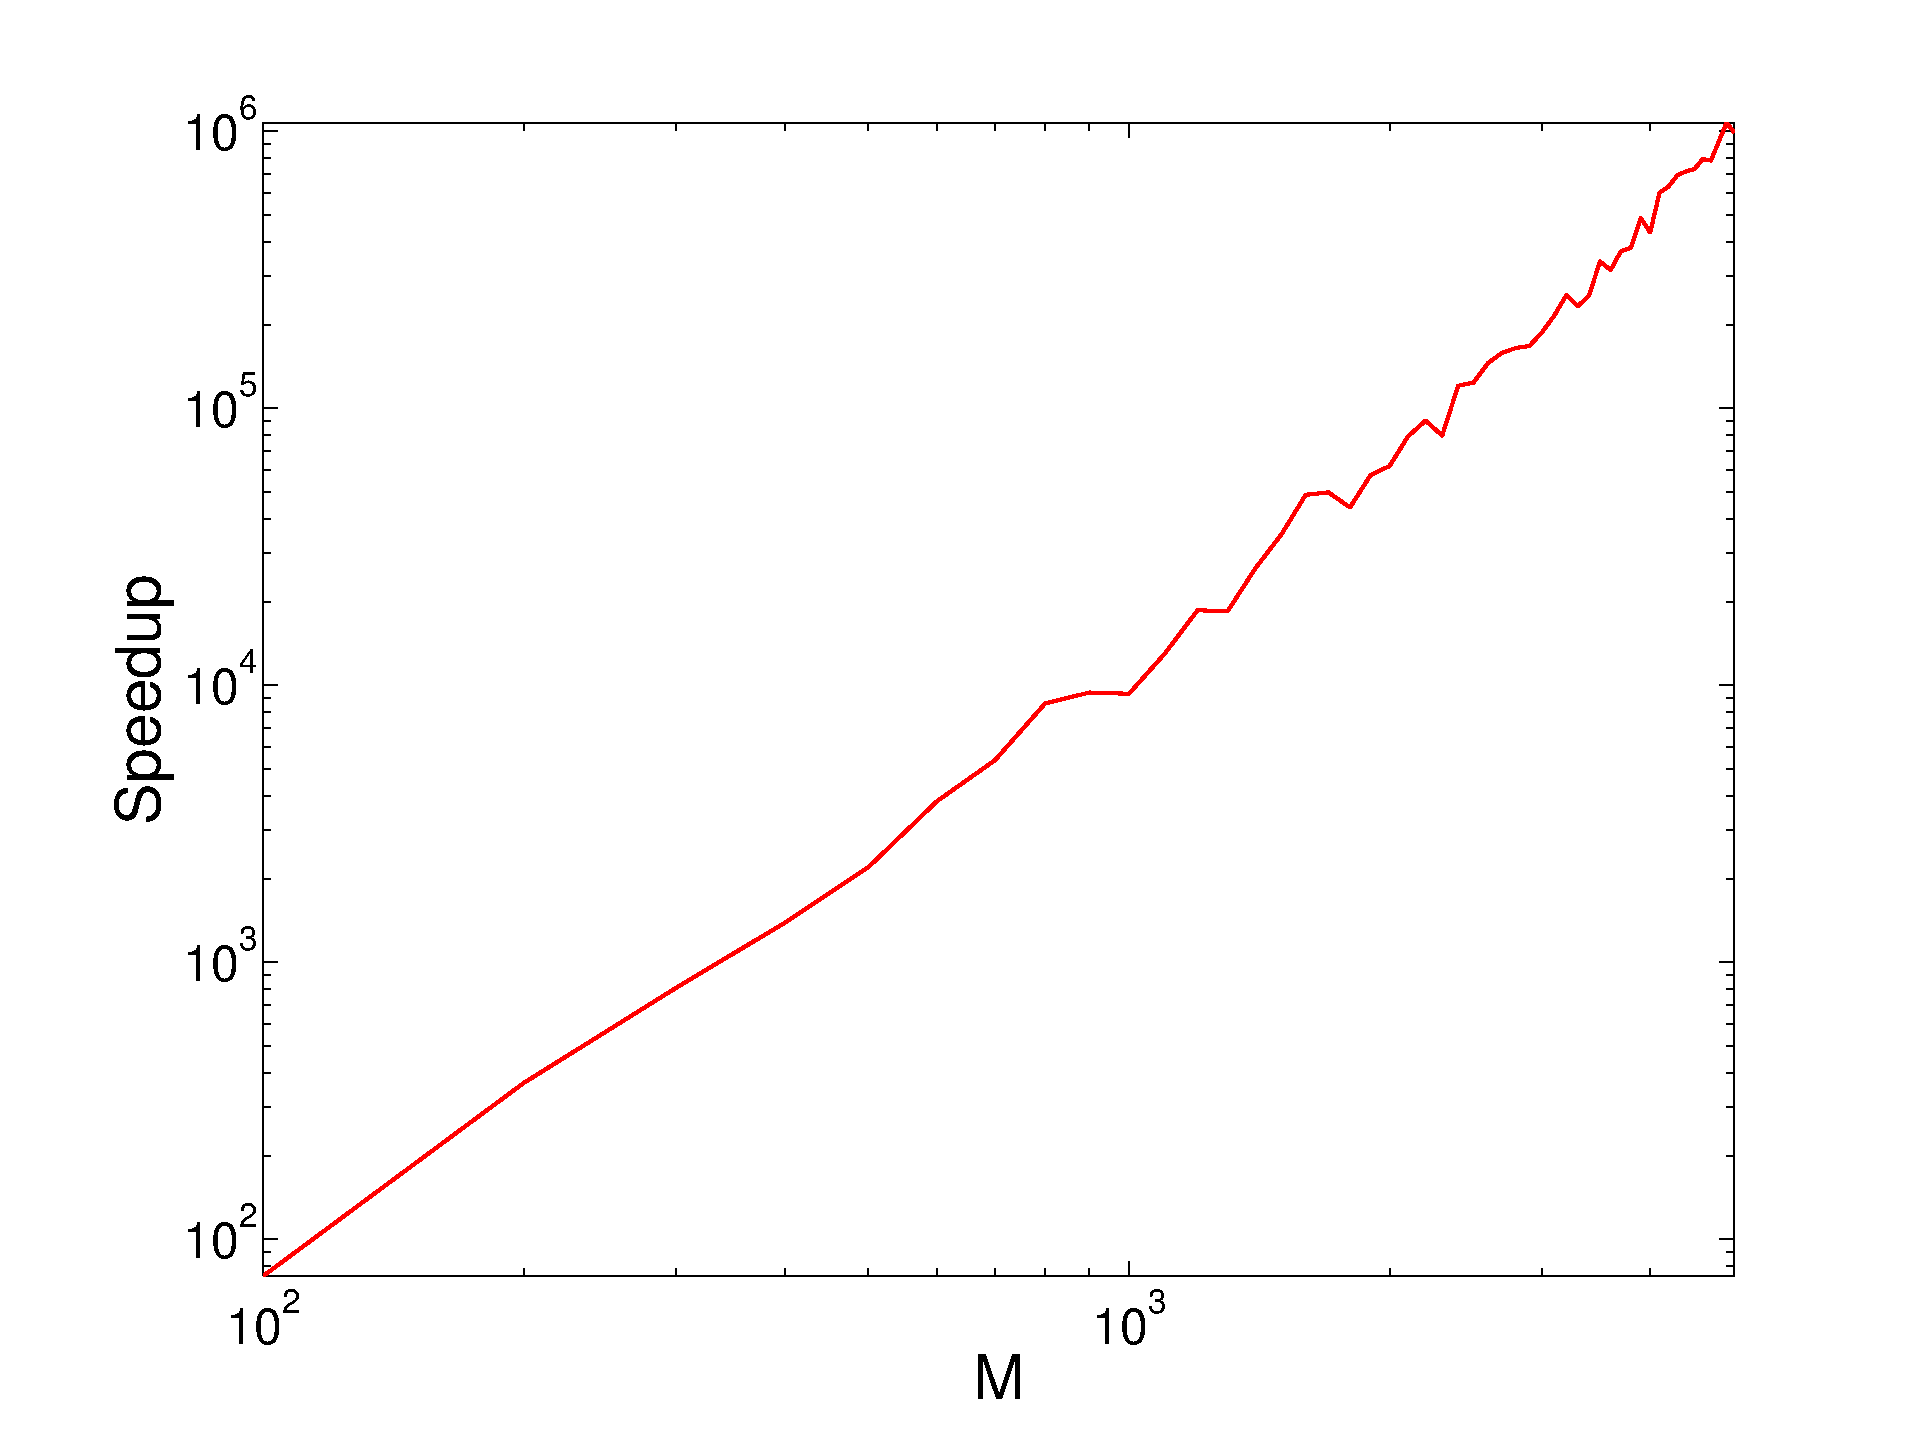
\includegraphics[width=0.7\textwidth,height=0.5\textwidth]{figMInvSpeedUp.eps}
  \vspace{1mm}
  \caption{Speedup of ODC framework prediction on either TGP or GPR while retrieving precomputed matrix inverses as $M$ increases, compared with computing them on test time by KNN scheme (log-log scale)}
  \label{fig:SpeedUp}
\end{minipage}
%\vspace{-10mm}
\end{figure*}
\begin{figure}
\centering
 \includegraphics[width=0.25\textwidth,height=0.2\textwidth]{Ekmeans57.png}
 \vspace{4mm}
\caption{Assign and Balance-EKmeans on 300,000 random 2D points, K= 57 (best seen electronically).}
\end{figure}
\end{comment}

Various approximation approaches have  been presented to reduce the computational complexity in the context of GPR. As detailed in \cite{park11}, approximation methods on Gaussian Processes may be categorized into three trends: matrix approximation,
likelihood approximation, and localized regression. The matrix approximation trend is inspired by the observation that the kernel matrix inversion is the major part of the expensive computation, and thus, approximating the matrix by a lower rank version, $M \ll N$\ignore{,   helps reduce the computational demand} (e.g.,  Nystr\"{o}m  Method~\cite{Nystrom01}). While this approach reduces the computational complexity from $O(N^3)$ to $O(N M^2)$ for training, there is no guarantee on the non-negativity of the predictive variance~\cite{Rasmussen:2005}. In the second trend,  likelihood approximation is performed on testing and training examples, given $M$ artificial examples known as inducing inputs, selected from the training set (e.g.,  Deterministic Training Conditional (DTC)~\cite{DTC03}, Full Independent conditional (FIC)~\cite{fic06}, Partial Independent Conditional (PIC)~\cite{pic07}). The drawback of this trend is \ignore{that it deals with }the dilemma of selecting $M$ inducing points, which might be distant from the test point, resulting in a performance decay; see Table~\ref{tab:thcomp} for the complexity of FIC.


\ignore{However, } A third trend, localized regression, is based on the belief that distant observations are almost unrelated\ignore{, and adopted in our work}. The prediction of a test point is achieved through its $M$ nearest points\ignore{ from the training set}. One technique to implement this notion is through decomposing the training points into disjoint clusters during training, where prediction functions are learned for  each of them~\cite{park11}. At test time, the prediction function of the closest
cluster\ignore{, where the test point belongs, } is used to predict the corresponding output. While this method is efficient\ignore{ and adaptive to non-stationary change}, it introduces discontinuity problems on boundaries of the subdomains. Another way to implement local regression is through Mixture of Experts (MoE) as an Ensemble method to make prediction based on computing the final output by combining outputs of local predictors called experts (see a study on MoE methods~\cite{tymoe12}). Examples include Bayesian committee
machine (BCM~\cite{BCM00}), local probabilistic regression (LPR~\cite{LPR08}), mixture of Tree of Gaussian Processes (GPs)~\cite{TreeGPs07}, and
Mixture of GPs~\cite{Rasmussen:2005}. While these approaches overcome the discontinuity problem by the combination mechanism, they suffer from intensive complexity at test time, which limits its applicability in large-scale setting\ignore{. One more computational aspect is that mixture models, as }, e.g., Tree of GPs and Mixture of GPs, involve complicated integration, approximated by computationally expensive sampling or Monte Carlo simulation. 

\ignore{
Park  et al~\citet{park11} proposed an approach for fast computation of GPR with a focus on large spatial data sets. The approach decomposes the domain of a single output regression function into small subdomains, inspired by a domain decomposition  approach for solving  Partial differential Equations (PDEs). It then infers a local regression function for each subdomain. In contrast to prior methods, this approach is easier to parallelize. However, it was mainly based on building consistent boundary value functions between subdomains on  a regular grid. Hence, their approach was evaluated on data of maximum input dimension $2$.}

Park etal.~\cite{park11} proposed a large-scale approach for  GPR by domain decomposition on up to 2D grid on input, where a local regression function is inferred for each subdomain such that they are consistent on boundaries.\ignore{The approach model the problem by solving Partial Differential Equations to maximize consistent prediction on the boundaries of sudomains, defined on a regular grid (upto 2D grid).} This approach obviously lacks a solution to high-dimensional input data because the size of the grid increases exponentially with the dimensions, which limits its applicability\ignore{makes the approach unapplicable in is not applicable to many applications}. More recently,\ignore{  Chalupka et al}~\cite{Chalupka:2013} proposed a Recursive Partitioning Scheme (RPC) to decompose the data into non-overlapping equal-size clusters, and they built a GPR on each cluster\ignore{; we denote this method as Local-RPC}. They showed that this local scheme gives better performance  than FIC~\cite{fic06} and other methods\ignore{ they compared with, in the time regimes as it operates}. However, this partitioning scheme obviously lacks consistency on the boundaries of the partitions and it was restricted to single-output GPR\ignore{, which limits its applicability in structured regression problems, e.g., human pose estimation}. Table~\ref{tab:thcomp} shows the complexity of this scheme denoted by local-RPC for GPR.
 
  
\begin{comment}
Another way to implement local regression is through Mixture of Experts (MoE)  as an Ensemble method to make prediction based on computing the final output by combining outputs of local predictors called experts (see a recent study of MoE approaches \cite{tymoe12}). Examples include Bayesian committee machine (BCM~\cite{BCM00}), local probabilistic regression (LPR~\cite{LPR08}), mixture of Tree of Gaussian Processes (GPs)~\cite{TreeGPs07}, and Mixture of GPs~\cite{Rasmussen:2005}. While these approaches overcome the discontinuity problem by the combination mechanism, they suffer from intensive complexity at test time, which limits its applicability in large-scale setting\ignore{. One more computational aspect is that mixture models, as } (e.g., Tree of GPs and Mixture of GPs, involve complicated integration, which is approximated by sampling or Monte Carlo simulation, that has a big computation cost).


, a common restriction in the prior work
\end{comment}





\begin{comment}
There have been increasing discriminative approaches to tackle pose reconstruction. These approaches were either based on nearest-neighbor schemes \cite{Shakhnarovich, Poppe07} or parametric predictors \cite{Rosales01learningbody, Agarwal06, Sminchisescu:2007}, trained using images of people and their corresponding 3d ground truth pose. A common drawback of these early approaches is that  they do not model the correlation between the outputs. This correlation  was successfully captured in~\cite{Bo:2010} by Twin Gaussian Processes (TGP). Yamada et al~\cite{Yamada:2012}  then proposed a covariance shift approach for TGP  to solve the data bias problem of the training data. In the remaining of this section, we focus on Twin Gaussian Processes work in~\cite{Bo:2010,Yamada:2012}.
\end{comment}

Beyond GPR, we found that local regression was adopted differently in structured regression models like Twin Gaussian Processes (TGP)~\cite{Bo:2010}, and also an data bias version of it, denoted by  IWTGP~\cite{Yamada:2012}.\ignore{ which deal with the data bias problem.In contrast to GPR, these models captures dependency between output dimensions, which leads to  better predictions in the Human 3D pose estimation task. } TGP and IWTGP outperform not only GPR in this task, but also various regression models including Hilbert Schmidt Independence Criterion (HSIC)~\cite{HSIC05}, Kernel Target Alignment (KTA)~\cite{KTA01}, and Weighted-KNN~\cite{Rasmussen:2005}. Both TGP and IWTGP have no closed-form expression for prediction. Hence, the prediction is made by gradient descent on a function that needs to compute the inverse of both the input and output kernel matrices, $O(N^3)$ complexity. Practically,  both approaches have been applied by finding the $M \ll N$ Nearest-Neighbors (NN) of each test  point in~\cite{Bo:2010} and~\cite{Yamada:2012}. The prediction of a test point is  $O(M^3)$ due to the inversion of $M \times M$ input and output kernel Matrices. \ignore{While this NN local regression scheme is one way to tackle the performance problem;} However, NN scheme has three drawbacks: (1) A regression model is computed for each test  point, which results in a scalability  problems in prediction (i.e., Matrix inversions on the NN of each each test point), (2) Number of neighbors might not be large enough to create an accurate prediction model since it is constrained by the first drawback, (3) It is inefficient compared with the other schemes used for GPR. Table~\ref{tab:thcomp} shows the complexity of this NN scheme\ignore{ denoted by NN}.
\ignore{
These drawbacks are overcome as a consequence of the six desirable properties. }

%------------------------------------------------------------------------- 
\section{ODC Framework}%
\label{sec:3}
\input{DDPrediction_v2}


\subsection{Training}
\label{sec:4}
\input{training2_v2}


\subsection{Prediction}
\label{sec:pred}

ODC-Prediction \ignore{under our  framework }is performed in  three steps. 
%\subsection{Finding the closest subdomains}
%\label{ss:fcc}

\noindent\textbf{{ (1) Finding the closest subdomains.}}
The closest  $K' \ll K$  subdomains  are determined based on the covariance norm of the displacement of  the test input from the means of the subdomain distribution (i.e. $\|\mathbf{x}-\boldsymbol{\mu
}'_{i} \|_{{\Sigma'_{i}}^{-1}}, i = 1: K$, where \ignore{$\boldsymbol{\mu
}'_{i}, {\Sigma'_{i}}^{-1}$ are as described in section ~\ref{sec:train2}),} $\|\mathbf{x}-\boldsymbol{\mu
}'_{i} \|_{{\Sigma'_{i}}^{-1}}$  = $ (\mathbf{x}-\boldsymbol{\mu
}'_{i})^T {\Sigma'_{i}}^{-1}  (\mathbf{x}-\boldsymbol{\mu
}'_{i})$. The reason behind using the covariance norm is that it captures details of the density of the distribution in all dimensions. Hence, it better models $p(\mathbf{x}|D_i)$, indicating better prediction of $\mathbf{x}$ on $D_i$.\ignore{, which indicates better prediction of corresponding $\mathbf{x}$ on $D_i$}
\ignore{
\begin{itemize}
\itemsep0em 
%\subsubsection{Mode 1} 
\item \textbf{Mode 1: } Closest clusters are determined based on the distance to the means of the clusters (i.e. $\|x-\mu_k \|, k = 1: NC$ ).
%\subsubsection{Mode 2}
\item \textbf{Mode 2: } This mode has an extra prediction parameter $M2K (Mode2 K)$. Algorithm ~\ref{alg:mode2FC}  details how closest clusters are selected in Mode 2.
%\subsubsection{Mode 3}
\item \textbf{Mode 3: } Closest clusters are determined based on the covariance norm of the displacement of  the test input from the means of the clusters (i.e. $\|x-\mu_{D_k} \|_{{\Sigma_{D_k}}^{-1}}, k = 1: NC$ . where $\mu_{D_k}, {\Sigma_{D_k}}^{-1}$ are as described in Algorithm ~\ref{alg:ddtgpm}), $\|x-\mu_{D_k} \|_{{\Sigma_{D_k}}^{-1}}$  = $ (x-\mu_{D_k})^T {\Sigma_{D_k}}^{-1}  (x-\mu_{D_k})$ 
\end{itemize}
}
\ignore{
\begin{algorithm}
\KwIn{query point X, DDTGPModel}
\KwOut{Closest subdomains }
Let $KNN_x =  KNN(x, X)$  \Comment{X is all input training points} \\
Let ${L_{KNN_x}} =  Clusters(KNN_x)$ \Comment{where Clusters($KNN_x$) returns the corresponding clusters for the returned points} \\ 
$FT = frequencyTable(L_{KNN_x})$ \Comment{where $frequencyTable(L_{KNN_x})$ returns an frequency of each clusters in $L_{KNN_x}$ }\\
$[sortedFT, sortedInd]  = sort(FT$) \\
$closestDomains = sortedInd[1:CDC] $\\ 
$closestFTS = sortedFT[1:CDC]$ \\
\caption{Mode 2 closest clusters algorithm}
\label{alg:mode2FC}
\end{algorithm}
}
%\subsection{Closest subdomains Prediction}
%\label{ss:csdp}


\noindent\textbf{{(2) Closest subdomains Prediction.}}
Having determined the closest subdomains, predictions are made for each of the closest clusters. We denote these predictions as ${\{Y^i_{x_*}\}}_{i=1}^{K'}$.  Each of these prediction are computed \ignore{by the following equation,} according to the selected kernel machine. For GPR, predictive mean and  variance are  $O(M\cdot d_X)\,$  and  $O(M^2 \cdot d_Y)\,$ respectively, for each output  dimension.  For TGP,   the prediction is  $O(l_2 \cdot M^2 \cdot d_Y)$; see Eq ~\ref{eq:tgp}. \ignore{, where $l_2$ is the number of iterations for  convergence, since TGP prediction has no closed form expression Similarly, any arbitrary kernel machine saves all factor of the prediction function that only depends on the training data.} \ignore{????? Add Example Kernel machines here????}
\begin{comment}
\textbf{GPR:}
\begin{equation}
\begin{split}
\hat{Y^i_{x_*}}_j = &\textbf{k}_{*_j}^T \mathcal{M}^i.(\textbf{K}_j + \sigma^2_{nj} \textbf{I})^{-1} \textbf{y}_j, \,\,
\sigma_{{Y^i_{x_*}}_j}^2  = k_{{**}_j} -\textbf{k}_{*_i}^T \mathcal{M}^i.(\textbf{K}^i_j + \sigma_{nj} \textbf{I})^{-1} \textbf{k}_{*_i})
\end{split}
\end{equation}
, where $\hat{Y^i_{x_*}}_j$ is the prediction output of the $j^{th}$ dimension at domain $i$.  Given $\mathcal{M}^i$ ,  $\hat{Y^i_{x_*}}_j$ and  $\sigma_{{Y^i_{x_*}}_j}^2$ are  $O(M)$  and  $O(M)^2$ respectively, for each dimension $j$.  

\textbf{TGP:}
\begin{equation}
\begin{split}
\hat{Y^i_{x_*}} =  \underset{Y^i_{x_*}}{\operatorname{argmin       }}[ & k_Y(Y^i_{x_*},Y^i_{x_*})  -2 k^i_y(Y_{x_*})^T \textbf{u}_i  -  \eta_i  log (k_Y(Y_{x_i},Y_{x_i})  -k^i_y(Y_{x_i})^T \mathcal{M}^i. ({\textbf{K}^i_Y}+ \lambda_y \textbf{I})^{-1}.  k^i_y(Y^i_{x_*}) ) ]
\end{split}
\end{equation}
where $\textbf{u}_i = \mathcal{M}^i.((\textbf{K}^i_X + \lambda^i_x  \textbf{I})^{-1}) \textbf{k}^i_x(\textbf{x}_*)$, $\eta  = K^i_X(\textbf{x}_*,\textbf{x}_*) -\textbf{k}(\textbf{x}_*)^T  \textbf{u} $.Given $\mathcal{M}^i$ , the $\hat{Y^i_{x_*}}_j$ has  $O(l_2 \cdot M)^2$ complexity, where $l_2$ is the number of iterations for  convergence of BFGS quasi-Newton gradient based optimizer. 
\end{comment}
\begin{comment}
\textbf{IWTGP:}
\begin{equation}
\begin{split}
\hat{Y^i_{x_*}} =  \underset{Y^i_{x_*}}{\operatorname{argmin       }}[ & k_Y(\textbf{Y}^i_{x_*},\textbf{Y}^i_{x_*}) -2 
k_y(\textbf{Y}^i_{x_*})^T \textbf{u}_w -\\ & \eta_w  log (K_Y(\textbf{Y}^i_{x_*},\textbf{Y}^i_{x_*}) -\\& 
k_y(\textbf{Y}^i_{x_*})^T {\textbf{W}^i}^\frac{1}{2} ({\textbf{W}^i}^\frac{1}{2} \textbf{K}_Y {\textbf{W}^i}^\frac{1}{2} +  \lambda_y I)^{-1} \\&{\textbf{W}^i}^\frac{1}{2} k_y(\textbf{Y}^i_{x_*}) ) ]
\end{split}
\end{equation}
where $\textbf{u}_w = \textbf{W}^\frac{1}{2}  (\textbf{W}^\frac{1}{2} \textbf{K}_X \textbf{W}^\frac{1}{2} + \lambda_x I)^{-1} \textbf{W}^\frac{1}{2} k_x(\textbf{x})$, $\eta_w = k_X(\textbf{x},\textbf{x}) - k_x(\textbf{x})^T \textbf{u}_w$. As detailed in section ~\ref{sec:train2}, $({\textbf{W}^i}^\frac{1}{2} \textbf{K}_X^i {\textbf{W}^i}^\frac{1}{2} + \lambda_x \textbf{I})^{-1}$,  $({{\textbf{W}^i}}^\frac{1}{2} \textbf{K}_X {\textbf{W}^i}^\frac{1}{2} + \lambda_x \textbf{I})^{-1}$ could be computed in quadratic time given  $\mathcal{M}^i$ and $W$. Hence,  the $\hat{Y^i_{x_*}}_j$ has  $O(l_d \cdot M)^2$ complexity, where $l_2$ is the number of iterations. 
\end{comment}
%\subsection{Subdomains weighting and Final prediction}
%\label{ss:sdw}

\noindent \textbf{{(3) Subdomains weighting and Final prediction.}}
The final predictions are formulated as $\textbf{Y}(x_*) = \sum_{i=1}^{K'} a_i \textbf{Y}^i_{x_*}, a_i>0, \sum_{i=1}^{K'} {a_i} =1 $. ${\{a_i\}}_{i=1}^{K'}$ are computed as follows.  Let the distribution of domain ${\{D^i_{x_*} = \|x-\mu'_{i} \|_{{\Sigma'_{k}}^{-1}}\}}_{i=1}^{K'}$ denotes to the distances to the closest subdomains, ${\{L^i_{x_*} = {1}/{D^i_{x_*}}\}}_{i=1}^{K'}$, $a_i ={L^i_{x_*}}/{\sum_{i=1}^{K'} {L^i_{x_*}}} $. \ignore{; see table ~\ref{tab:thcomp} for detailed complexity of the ODC framework in GPR and TGP. }


It is not hard to see that when $K' = 1$, the prediction step reduces to regression using the closest subdomain to the test point. However it is  reasonable in most of the prior work to make prediction using the closest model, we generalized it to $K'$ closest kernel machines and combining their predictions,  so as to study how consistency of the combined prediction behaves as the overlap increases (i.e., $p$); see the experiments.\ignore{ Table ~\ref{tab:thcomp} illustrates the computational complexity of the framework. }


% Table generated by Excel2LaTeX from sheet 'Sheet1'


\ignore{\begin{itemize}
\itemsep0em 
%\subsubsection{Mode 1} 
\item \textbf{Mode 1: } Let ${\{D_{x_i}\}}_{i=1}^{CDC}$ denotes to the distances to the closest clusters, ${\{L_{x_i} = \frac{1}{D_{x_i}}\}}_{i=1}^{CDC}$. Then $W_i =\frac{L_x(i)}{\sum_{i=1}^{CDC} {L_x(i)}} $
\item \textbf{Mode 2: }$W_i = \frac{closestFTS(i)}{\sum_{i=1}^{CDC} closestFTS(i)}$
 where closestFTS is as computed in subsection ~\ref{ss:fcc}.
\item \textbf{Mode 3: } Let ${\{D_{x_i} = \|x-\mu_{D_k} \|_{{\Sigma_{D_k}}^{-1}}\}}_{i=1}^{CDC}$ denotes to the distances to the closest clusters, ${\{L_{x_i} = \frac{1}{D_{x_i}}\}}_{i=1}^{CDC}$. Then  $W_i =\frac{L_x(i)}{\sum_{i=1}^{CDC} {L_x(i)}} $.
\end{itemize}}
\ignore{
noindent \textbf{Computational Complexity:} Overall computational complexity of the prediction = $O( n_{Tst}* CDC * (\frac{N_{Tr}}{NC}) ^2)$ (i.e. quadratic complexity) which is significantly better than cubic complexity of the original TGP model. where $n_{Tst}$ is the number of the test points, $N_{Tr}$ is the number of points in the training data.
\subsection{Data Bias handling ($CovShift$ Flag = $True$)}
\input{databias}}

\section{Experimental Results}
\label{sec:6}
\input{experiments_v2}

\section{Conclusion}
\label{sec:7}
We proposed an efficient ODC framework for kernel machines and validated the framework on structured regression machines on three human pose estimation datasets. The key idea is to equally  partition the data and create cohesive overlapping subdomains, where local kernel machines are computed for each of them. The framework is general and could be applied to various kernel machine beyond GPR, TGP, IWTGP validated in this work. Similar to TGP and IWTGP, our framework could be easily applied to the recently proposed Generalized  TGP~\cite{SMTGP_Elhoseiny15} which is based on Sharma Mittal divergence, a relative entropy measure brought from Physics community. We also theoretically justified  our framework's notion. 

\noindent \textbf{Acknowledgment.} This research was partially funded by NSF award \# 1409683.


\ignore{In this paper, we presented an ODC framework for structured regression kernel machines including GPR and TGP, applied to  3D pose estimation. The proposed model preserves accuracy while achieving a significant speedup in prediction, which is crucial for large scale prediction problems. The approach was evaluated on Poser, Human Eva and Human3.6M datasets. The key idea is to equally  partition the data and create cohesive overlapping subdomains, where local kernel machines are computed for each of them. The final prediction is then computed the predictions of the closest kernel machines. We should some interesting properties of the proposed framework including its applicability to a variety of the state-of the-art kernel methods.}

%\begin{abstract}
%\input{abstract}
%\keywords{Text Visualization \and Multi-level MindMap Automation}
%\end{abstract}



%%%%%%%%% BODY TEXT

%\section{Kernel Conclusion}
%\input{Kconclusion}

%\bibliographystyle{ACM-Reference-Format-Journals}



%\begin{acknowledgements}
%If you'd like to thank anyone, place your comments here
%and remove the percent signs.
%\end{acknowledgements}

% BibTeX users please use one of
%\bibliographystyle{spbasic}      % basic style, author-year citations
\bibliographystyle{spmpsci}      % mathematics and
%\bibliography{acmsmall-sample-bibfile}
%\bibliography{write_a_classifier}
\bibliography{egbib.bib}

\begin{appendices}


\section{IWTGP-ODC Experiments}
Tables ~\ref{tab:poserw} and ~\ref{tab:hevaresw} details the results of IWTGP-ODC experiments on Poser and HumanEva datasets in terms of error and speedup in prediction time.


\begin{table}[htbp]
  \centering
    \scalebox{0.8}
  {
     \begin{tabular}{|c|cc|}
      \hline
    \multirow{2}[4]{*}{\textbf{}} & \textbf{IWTTGP} & \multicolumn{1}{c|}{\textbf{IWTGP-ODC}} \\
     	& ($M = 800, M_{tst} = 418$)  & ($M = 800, M_{tst} = 418$)	\\ \hline
    \textbf{error (deg)} & 6.1 &  5.32 \\
    \textbf{err reduction (deg)} & -     &  \textbf{0.783 }\\
    \textbf{err reduction \%} & -     & \textbf{12.836\%} \\
    \textbf{Prediction Time (sec)} & 360.0  & 26.61 \\
    \textbf{speedUp} & -      & \textbf{13.5} \\ \hline
    \end{tabular}%     
    }
  \caption{POSER dataset IWTGP-NN vs  IWTGP-ODC}
 \label{tab:poserw}%
\end{table}%

\begin{table}[htbp]
  \centering
  \scalebox{0.9}
  {
\begin{tabular}{|c|cc|}
\hline
    \multirow{2}[4]{*}{\textbf{}} & \textbf{IWTGP} & \multicolumn{1}{c|}{\textbf{IWTTGP-ODC}} \\
    & ($M = M_{tst} = 800$)& ($M=M_{tst}=800$)\\  \hline
          & \textbf{}  & \textbf{ } \\
    \textbf{error (mm)} & 39.1  & 39.3 \\
    \textbf{err reduction (mm)} & -     & \textbf{\textbf{-0.2}} \\
    \textbf{err reduction \%} & -   & \textbf{\textbf{-0.512\%}} \\
    \textbf{Prediction Time (sec)} & 7938.15 &  569.66 \\
    \textbf{speedUp} & -     &  \textbf{13.92}\\ \hline
    \end{tabular}%
    }
 \caption{Humen Eva dataset: IWTGPKNN vs IWTGP-ODC}
  \label{tab:hevaresw}
\end{table}%




%\section{More Figures and Results}
%figure ~\ref{fig:ODCAnalysis400} shows our analysis on ODC for M =400. 

\ignore{
\begin{figure}[h!]
\centering
\begin{tabular}{c}
\bmvaHangBox{{  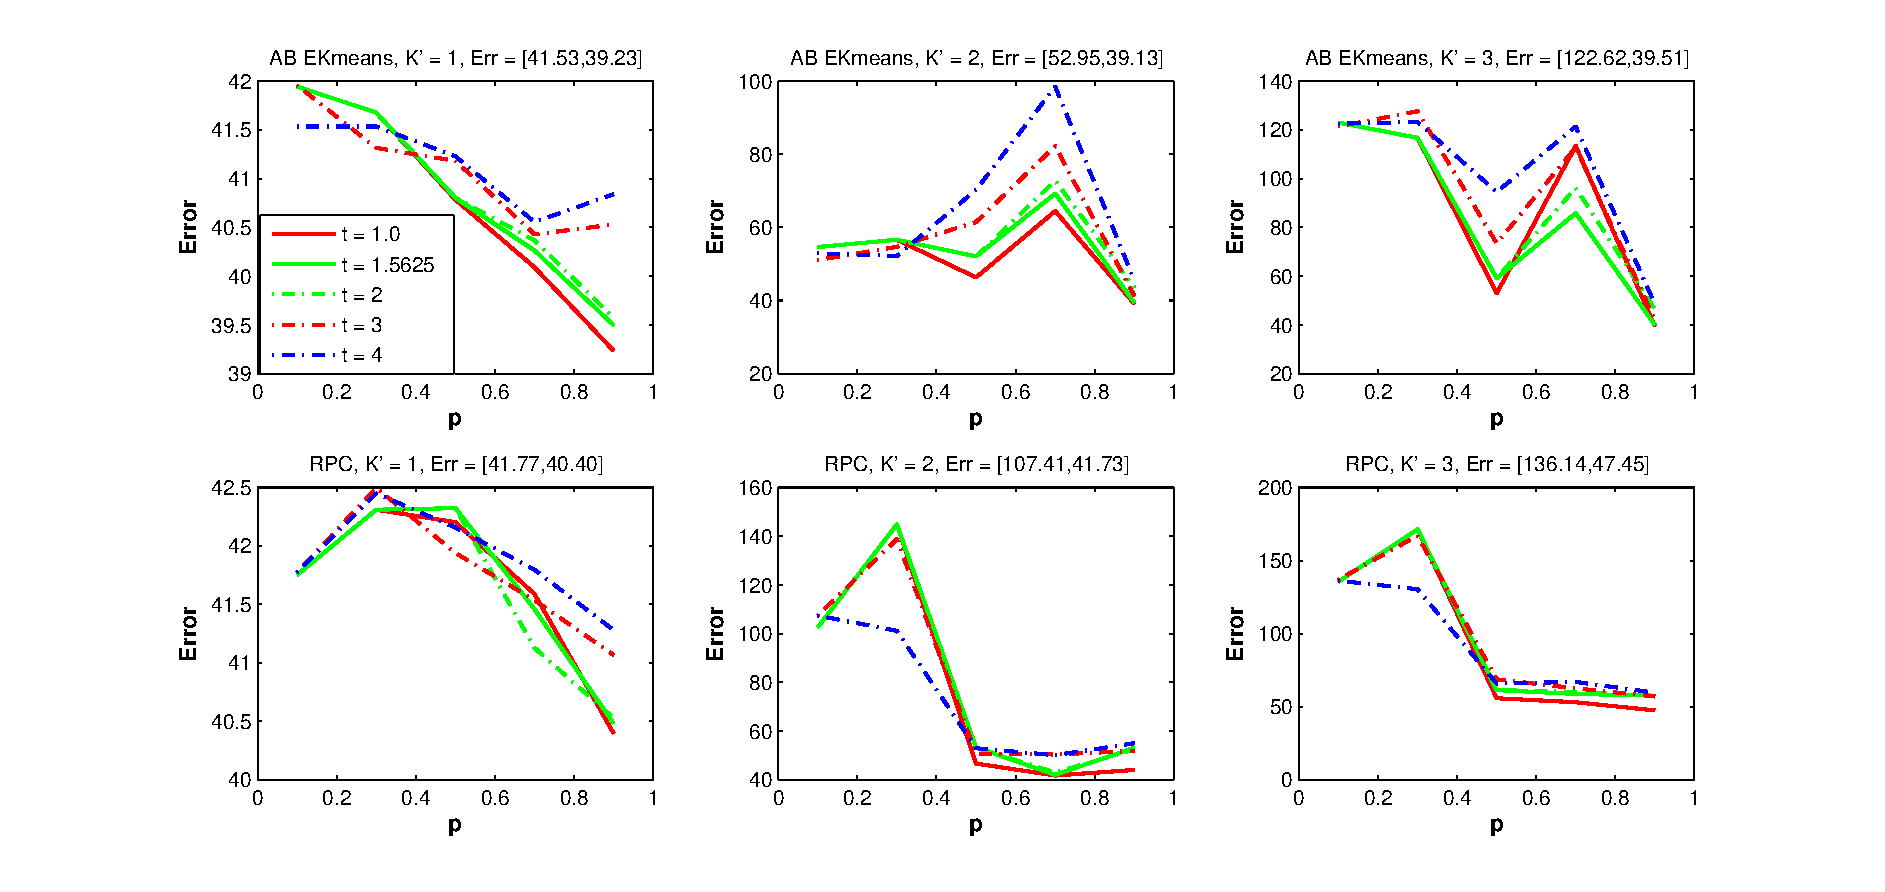
\includegraphics[width=1.0\textwidth,height=0.34\textwidth]{figTGP400HEva2.eps}}}\\
(a) TGP-ODC (M=400) \\
\bmvaHangBox{{  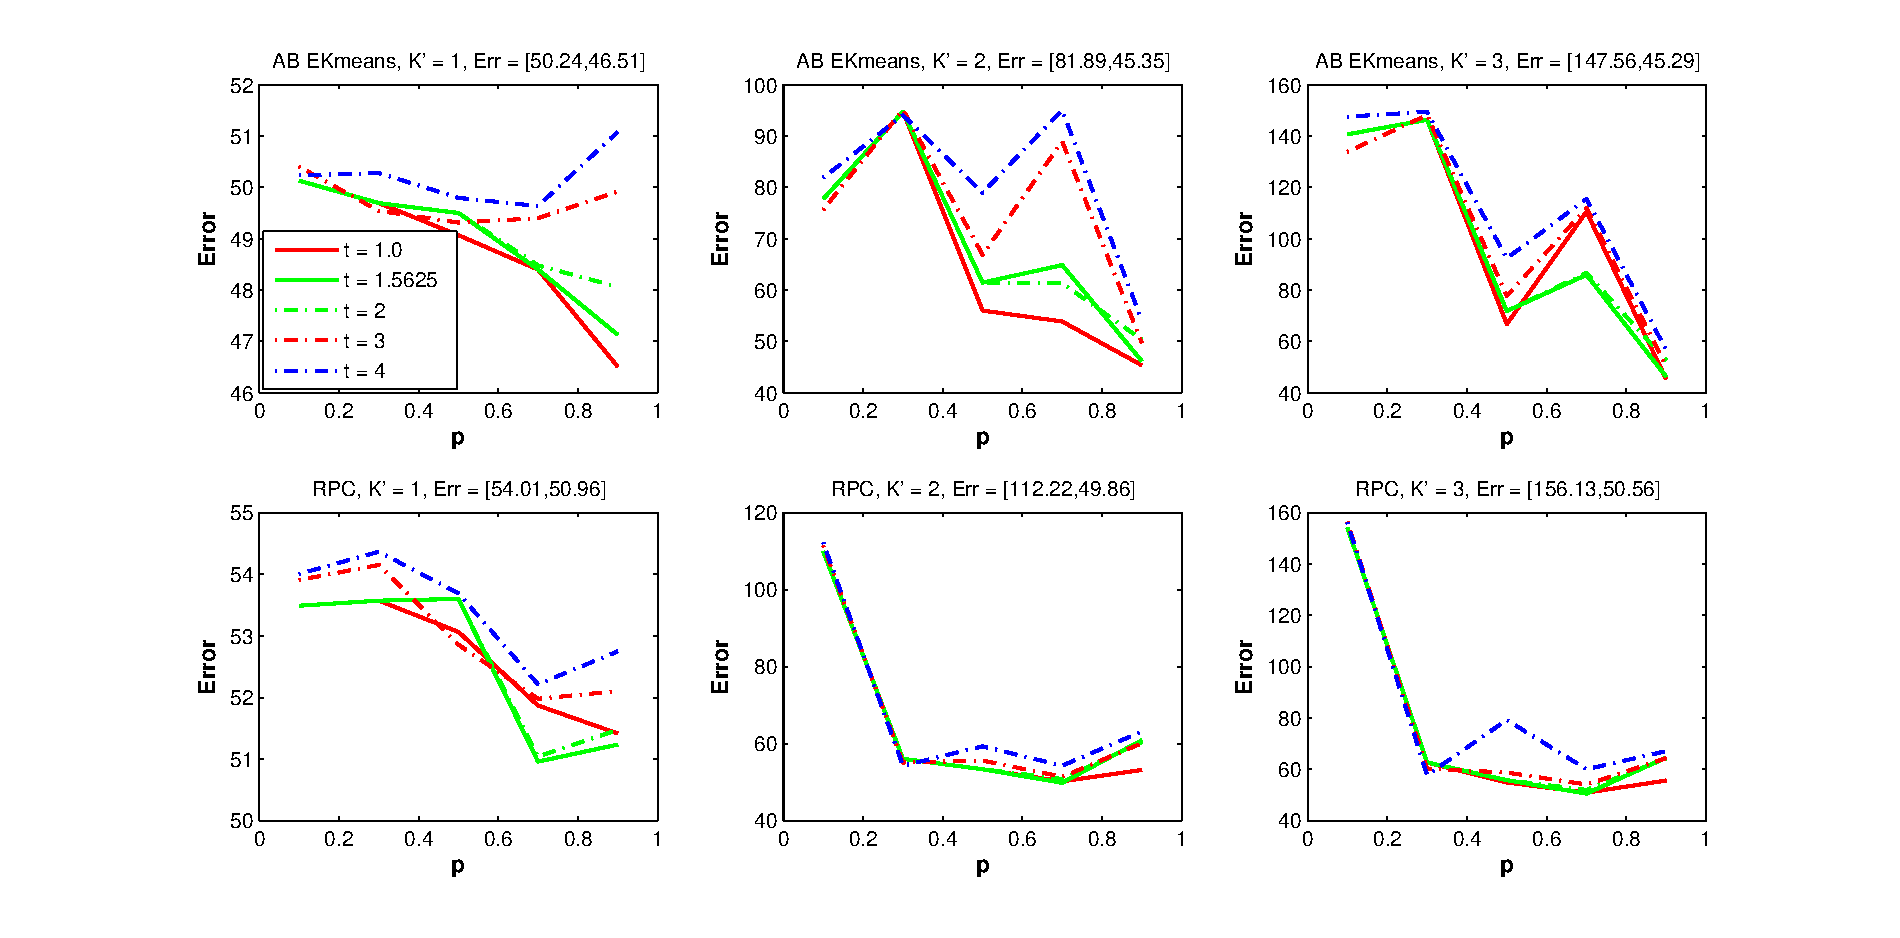
\includegraphics[width=1.0\textwidth,height=0.34\textwidth]{figGPR400HEva2.eps}}}\\
(a) GPR-ODC (M=400) \\
\end{tabular}
\vspace{2mm}
\caption{Overlapping Domain Cover Parameter Analysis of GPR and TGP  on Human Eva Dataset (best seen in color) (M=400)}
\label{fig:ODCAnalysis400}
%\label{fig:teaser}
\end{figure}}


\begin{comment}
\begin{table*}[htbp!]
  \centering
      \vspace{4pt}
  \caption{Error and Time for Poser and Human Eva datasets (on 2.6GHZ intel core i7), M = 800}
    \vspace{3pt}
    \scalebox{0.8}{
    \begin{tabular}{|l|l|lll|lll|}%ccc}
    \toprule
          &   & \textbf{Poser} & \textbf{} &       & \textbf{HumanEva} &       &      \\% & \textbf{Human 3.6} &       &  \\
    \midrule
         & & \textbf{Error (deg)} & \textbf{Training Time} & \textbf{Prediction Time} & \textbf{Error (mm) } & \textbf{Training Time} & \textbf{Prediction Time} \\%& \textbf{Error} & \textbf{Training Time} & \textbf{Prediction Time} \\
 \textbf{TGP}   & \textbf{NN} & 5.43       &  -     &    188.99 sec   & \textbf{38.1}      &  -     & 6364 sec \\%       &       &       &  \\
  & \textbf{ODC ($p= 0.9, t=1, K'=1$)-Ekmeans} & \textbf{5.4 }     &      (3.7 +25.1 ) sec  &   \textbf{16.5}  sec  &    \textbf{38.99 }  &  (2001 + 45.4) sec    &  \textbf{298} sec\\%       &       &       &  \\
    & \textbf{ODC ($p= 0.9, t=1, K'=2$)-Ekmeans} & {5.53}     &      (3.7 +29.4 ) sec  &   47.04  sec  &    {39.2 }  &  (2001 + 45.24) sec    &  569.6946  sec\\%       &       &       &  \\
      & \textbf{ODC ($p= 0.9, t=1, K'=3$)-Ekmeans} & {5.4}     &      (3.7 +28.8 ) sec  &   71.4 sec  &    {40.9 }  &  (2001 +  45.7) sec    &  721.0 sec\\%       &       &       &  \\
    & \textbf{ODC ($p= 0, t=1, K'=1$)-Ekmeans} &   7.6    &    (3.9 + 1.33) sec   &   14.8 sec  &    41.87   & (240 + 4.9832 ) sec       &  256.7 \\%      &       &       &  \\
       & \textbf{ODC ($p= 0, t=1, K'=2$)-Ekmeans} &   12.3    &    (3.9 + 2.69) sec   &   42.25 sec  &    136.52 & (240 + 4.7790  ) sec       &  514.93 \\%      &       &       &  \\
       & \textbf{ODC ($p= 0, t=1, K'=3$)-Ekmeans} &   12.52    &    (3.9 + 1.86) sec   &    72.38 sec  &    187.72   & (240 + 4.75 ) sec       &  771 \\%      &       &       &  \\
      &  \textbf{ODC ($p= 0.9, t=1, K'=1$)-RPC} & 5.6      &      (0.23 +41.6 ) sec  &   15.8 sec  &   39.9  &    ( 0.45 + 49.05) sec     & 277.25 sec\\%       &       &       &  \\
         &  \textbf{ODC ($p= 0.9, t=1, K'=2$)-RPC} & 5.52      &      (0.23 +43.80 ) sec  &   43.802 sec  &   40.41  &    ( 0.45 + 46.77) sec     & 677.52 sec\\%       &       &       &  \\
        &  \textbf{ODC ($p= 0.9, t=1, K'=3$)-RPC} & 5.59  &      (0.23 +43.05 ) sec  &   67.11 sec  &    41.21&    ( 0.45 + 47.63) sec     &  883 sec\\%       &       &       &  \\
  &  \textbf{ODC ($p= 0, t=1, K'=1$)-RPC} &   7.7    &   (0.15 + 1.7) sec   &   13.89 sec  &  42.32    &  (0.19 + 5.3)      sec &  241.64 sec\\%      &       &       &  \\
    &  \textbf{ODC ($p= 0, t=1, K'=2$)-RPC} &   9.29 &   (0.15 + 1.8) sec   &   41.86 sec  &  58.99    &  (0.19 + 5.16)      sec &  475.14 sec\\%      &       &       &  \\
      &  \textbf{ODC ($p= 0, t=1, K'=3$)-RPC} &   12.47    &   (0.15 + 1.80) sec   &   66.42 sec  &  136    &  (0.19 + 5.2)      sec &  721.49 sec\\%      &       &       &  \\
      \hline
  \textbf{GPR}  & \textbf{NN} & 6.77      &   -    &  24 sec     &   54.8    &      - &    618  sec \\%&       &       &  \\
   & \textbf{ODC ($p= 0.9, t=1 , K'=1$)-Ekmeans} &  \textbf{6.27}      &  (3.7 +11.1 ) sec  &       \textbf{0.56}  sec & \textbf{49.3}  &   (2001 + 42.85)sec & \textbf{78.85} sec \\%       &       &       &  \\
   & \textbf{ODC($p= 0.0, t=1 , K'=1$)-Ekmeans} & 7.54      &   ( 3.9 + 1.38 sec) &    0.35 sec   & 49.6  &  (240 + 6.4) sec  &  48.1 sec\\%      &       &       &  \\
  & \textbf{ODC ($p= 0.9, t=1 , K'=1$)-RPC} &  6.45      &  (0.23 +17.3 ) sec  &       0.52  sec & 52.8  & (0.49 + 46.06) sec     &  64.13 sec\\%       &       &       &  \\
    & \textbf{ODC ($p= 0.0, t=1 , K'=1$)-RPC  = ~\cite{Chalupka:2013}} &   7.46    &   (0.15 + 1.47) sec &    0.27 sec   & 54.6  &  (0.261 + 4.58 ) sec & 43.52 sec\\%      &       &       &  \\
    & \textbf{FITC ~\cite{fic06}} &   7.63 (+/- 0.4)  &   (- + 20.63)   &    0.3106     &   68.36(+/- 0.84)    &  -     & 101.5442 (+/- 1.36) sec\\%      &       &       &  \\
    \bottomrule
    \end{tabular}}%
  \label{tab:tblRes_detailed}%
\end{table*}%
\end{comment}


\section{More figures on AB Ekmeans}





 Figure~\ref{fig:ekmeans} shows the clustering performance on 300000 random 2D point (K=5). Figure  ~\ref{fig:hevaVis3} shows the clustering output of our algorithm visualized on using the first three principal components of Human Eva training hog features. The figures shows that the cluster are spatially cohesive but not necessarily circular. This makes the elliptic distribution of the data captured by Mode 3 gives more accuracy membership measure me to the subdomains. %\ignore{That's why Mode 3 gives a better accuracy than Mod 1. It also gives an accuracy better than Mode 2. A problem in Mode 2 is how to choose K so that it relects the correct associativity of the test point to the closest subdomans.}
 
 \ignore{\begin{figure}[h!]
\begin{tabular}{ccc}
\bmvaHangBox{\fbox{\includegraphics[width=4.6cm]{Ekmeans5.png}}}&
\bmvaHangBox{\fbox{\includegraphics[width=5.2cm]{Ekmeans57.png}}}\\
(a)&(b)
\end{tabular}
\caption{Applying our Assign and Balance variant of Kmeans on 300,000 random 2D points:  5 clusters}
\label{fig:ekmeans}
%\label{fig:teaser}
\end{figure}}
 

 \begin{figure}[h!]
 \centering
\begin{subfigure}[b]{0.5\textwidth}
\includegraphics[width=6.6cm]{Ekmeans5.png}
  \caption{5 clusters}
\end{subfigure}
%\begin{subfigure}[b]{0.5\textwidth}
%\includegraphics[width=5.2cm]{Ekmeans57.png}
  %\caption{57 clusters}
%\end{subfigure}
\caption{Applying our Assign and Balance variant of Kmeans on 300,000 random 2D points}
\label{fig:ekmeans}
%\label{fig:teaser}
\end{figure}
\begin{figure}[h!]
\centering
 \includegraphics[width=0.5\textwidth]{HumanEVAPCAVis.jpg}
\caption{Human Eva clustering first three Pricipal Components }
\label{fig:hevaVis3}
\end{figure}


%\subsection{Equal Size Assignment Algorithms Pseudocode}
%As presented in the pape, our k-means variant algorithms modifies only the assignment step of  the standard k-means algorithm. Algorithm ~\ref{alg:ddclusterALg2} and ~\ref{alg:ddclusterALg1} shows the pseudo-code of the assignments steps on IMDA-k-means and AB-k-means algorithms respectively. We attach the MATLAB implementation of both algorithms in "Ekmeans-assign" folder, We plan to release the whole implementation of our paper as well as soon as we well-document of the code. 




\section{Overlapping Domain Cover(ODC) Generation-Algorithm}

Algorithm ~\ref{alg:sdgen} shows how the overlapping sub-domains are generated form the the equal size clusters from the closest $r$ clusters. \ignore{ if the retrieved nearest neighbor points  belongs to more than $^OC_C$ clusters.}
\begin{algorithm}
{\textbf{Input:} Clusters ${\{C_k\}}_{k=1}^{K} $}
\KwOut{Overlapping subdomains ${\{D_k\}}_{k=1}^{K}$}
\ForEach{Cluster $C_k$}{
Compute the closest $r$ clusters ${\{{{C^{'}}_i}\}}_{i=1}^{r}$ based on $DK_i = \| \mu_k- \mu_i \|$ , $i\neq k$\\
Let $LK_i = 1/DK_i,  {WK_i} =  \frac{LK_i}{\sum_{l=1}^{^OC_C} LK_l}$  ${i=1 : r}$\\
Let ${NPK_i} =  floor(WK_i * OPC)$, ${i=1 : r}$ \\
Let $ExKPts = (1-p) M - \sum_{l=1}^{r} NPK_l$ \\
Let ${NPK_i}$ =  $NPK_i +1$ , $ i=1 : ExKPts $\\
$D_k =  C_k$ \\
Let $overflow = 0$\\
  \Comment{The following for loop goes over the $r$ clusters on an increasing order of $DK_i$ }\\
\For{i=1 : $r$} {
  \If{${NPK_i}$> $|C_i|$} { $overflow = overflow+ {NPK_i} -|C_i|$ \\  $NPK_i = |C_i|$   } 
  \If{${NPK_i}$< $|C_i|$} { $G_i =min(overflow, |C_i| -NPK_i$ ) \\  $NPK_i = NPK_i +G_i $ \\  $overflow =overflow-G_i$   } 
  %\ELSE{} {}\\
 $Ps_i = KNN({OVC_K}_j,NPK_i )$ 
 \\ $D_k = D_k \cup Ps_i$ 
 }


\For{i=1 : $r$} { $Ps_i = KNN({OVC_K}_j,NPK_i )$ \\ $D_k = D_k \cup Ps_i$ }

\Comment{where KNN is the K-nearest neighbors algorithms. For high performance calculation of $KNN$, we use FLANN \cite{flann09} to calculate $KNN$.}
}
\caption{Subdomains Generation (Note: All ${\{D_k\}}_{k=1}^{K}$ are stored as indices to $X$).  }
\label{alg:sdgen}
\end{algorithm}





%
%
%
%\subsection{Prediction} 
%From the above discussion, the prediction for each subdomain is computed as follows
%
%\begin{equation}
%\begin{split}
%\hat{Y^i_{x_*}} =  \underset{Y^i_{x_*}}{\operatorname{argmin       }}[ & k_Y(\textbf{Y}^i_{x_*},\textbf{Y}^i_{x_*}) -2 
%k_y(\textbf{Y}^i_{x_*})^T \textbf{u}_w -\\ & \eta_w  log (K_Y(\textbf{Y}^i_{x_*},\textbf{Y}^i_{x_*}) -\\& 
%k_y(\textbf{Y}^i_{x_*})^T {\textbf{W}^i}^\frac{1}{2} ({\textbf{W}^i}^\frac{1}{2} \textbf{K}_Y {\textbf{W}^i}^\frac{1}{2} +  \lambda_y I)^{-1} \\&{\textbf{W}^i}^\frac{1}{2} k_y(\textbf{Y}^i_{x_*}) ) ]
%\end{split}
%\end{equation}
%
%where $\textbf{u}_w = \textbf{W}^\frac{1}{2}  (\textbf{W}^\frac{1}{2} \textbf{K}_X \textbf{W}^\frac{1}{2} + \lambda_x I)^{-1} \textbf{W}^\frac{1}{2} k_x(\textbf{x})$, $\eta_w = k_X(\textbf{x},\textbf{x}) - k_x(\textbf{x})^T \textbf{u}_w$, $({\textbf{W}^i}^\frac{1}{2} \textbf{K}_X^i {\textbf{W}^i}^\frac{1}{2} + \lambda_x \textbf{I})^{-1}$,  $({{\textbf{W}^i}}^\frac{1}{2} \textbf{K}_X {\textbf{W}^i}^\frac{1}{2} + \lambda_x \textbf{I})^{-1}$ could be computed in quadratic time given  $\mathcal{M}^i$ and $W$. Hence,  the $\hat{Y^i_{x_*}}_j$ has  $O(iters \cdot M)^2$ complexity, where $iters$ is the number of iterations. 



\section{Local Kernel Machines hyper-parameters on each dataset}
The hyper parameters were learnt using cross validation on the training set for  GPR, TGP and IWTGP that we are interested in. The following subsection present the learnt hyper-parameters and the error measures on each dataset in case of TGPs.
\subsection{Poser Dataset}
The parameters $2 \rho_x^2$, $2 \rho_y^2$, $\lambda_X$, and $\lambda_Y$ were assigned to  $5$, $5000$, $10^{-4}$, and $10^{-4}$, respectively. 

\subsection{HumanEva Dataset}

The parameters $2 \rho_x^2$, $2 \rho_y^2$, $\lambda_X$, and $\lambda_Y$ were assigned to  $5$, $500000$, $10^{-3}$, and $10^{-3}$, respectively. 


\subsection{Human 3.6 Dataset}

The parameters $2 \rho_x^2$, $2 \rho_y^2$, $\lambda_X$, and $\lambda_Y$ were assigned to  $5$, $500000$, $10^{-3}$, and $10^{-3}$, respectively.




%\section{Equal Size Kmeans (EKmeans): More Details}



\end{appendices}

\clearpage
%begin{comment}
\begin{wrapfigure}{l}{0.2\textwidth}
     \includegraphics[width=0.2\textwidth]{elhoseiny.jpg}
\end{wrapfigure}
\textbf{Mohamed Elhoseiny } is a PostDoc Researcher at Facebook Research.
His primary research interest is in computer vision, machine learning, intersection between natural language and vision, language guided visual-perception,  and visual reasoning, art \& AI. He received his PhD degree from Rutgers University, New Brunswick, in 2016 under Prof. Ahmed Elgammal. Mohamed received an NSF Fellowship in 2014 for the Write-a-Classifier project (ICCV13), best intern award at SRI International 2014, and the Doctoral Consortium award at CVPR 2016.
\vspace{2mm}
 \begin{wrapfigure}{l}{0.2\textwidth}  
\vspace{-5mm} 
         \includegraphics[width=0.2\textwidth]{elgammal.jpg}
         \vspace{-10mm} 
\end{wrapfigure}\,\,\;

 \textbf{Ahmed Elgammal} is a professor at the Department of Computer Science, Rutgers, the State University of New Jersey Since Fall 2002. Dr. Elgammal is also a member of the Center for Computational Biomedicine Imaging and Modeling (CBIM). His primary research interest is computer vision and machine learning. His research focus includes human activity recognition, human motion analysis, tracking, human identification, and statistical methods for computer vision. Dr. Elgammal received the National Science Foundation CAREER Award in 2006. Dr. Elgammal has been the Principal Investigator and Co-Principal Investigator of several research projects in the areas of Human Motion Analysis, Gait Analysis, Tracking, Facial Expression Analysis and Scene Modeling; funded by NSF and ONR. Dr. Elgammal is Member of the review committee/board in several of the top conferences and journals in the computer vision field. Dr. Elgammal received his Ph.D. in 2002 from the University of Maryland, College Park. He is a senior IEEE member. 

%\end{comment}
\begin{comment}
\begin{biography}[me.eps]{Mohamed Elhoseiny}
 is a PostDoc Researcher at Facebook Research.
His primary research interest is in computer vision, machine learning, intersection between natural language and vision, language guided visual-perception,  and visual reasoning, art \& AI. He received his PhD degree from Rutgers University, New Brunswick, in 2016 under Prof. Ahmed Elgammal. Mohamed received an NSF Fellowship in 2014 for the Write-a-Classifier project (ICCV13), best intern award at SRI International 2014, and the Doctoral Consortium award at CVPR 2016.
\end{biography}

\begin{biography}[elgammal2.eps]{Ahmed Elgammal}
is an associate professor at the Department of Computer Science, Rutgers, the State University of New Jersey Since Fall 2002. Dr. Elgammal is also a member of the Center for Computational Biomedicine Imaging and Modeling (CBIM). His primary research interest is computer vision and machine learning. His research focus includes human activity recognition, human motion analysis, tracking, human identification, and statistical methods for computer vision. Dr. Elgammal received the National Science Foundation CAREER Award in 2006. Dr. Elgammal has been the Principal Investigator and Co-Principal Investigator of several research projects in the areas of Human Motion Analysis, Gait Analysis, Tracking, Facial Expression Analysis and Scene Modeling; funded by NSF and ONR. Dr. Elgammal is Member of the review committee/board in several of the top conferences and journals in the computer vision field. Dr. Elgammal received his Ph.D. in 2002 from the University of Maryland, College Park.
\end{biography}
\end{comment}

\end{document}
% end of file template.tex

